\begin{figure}[t]
  \vspace{-1.0em}
  \centering
  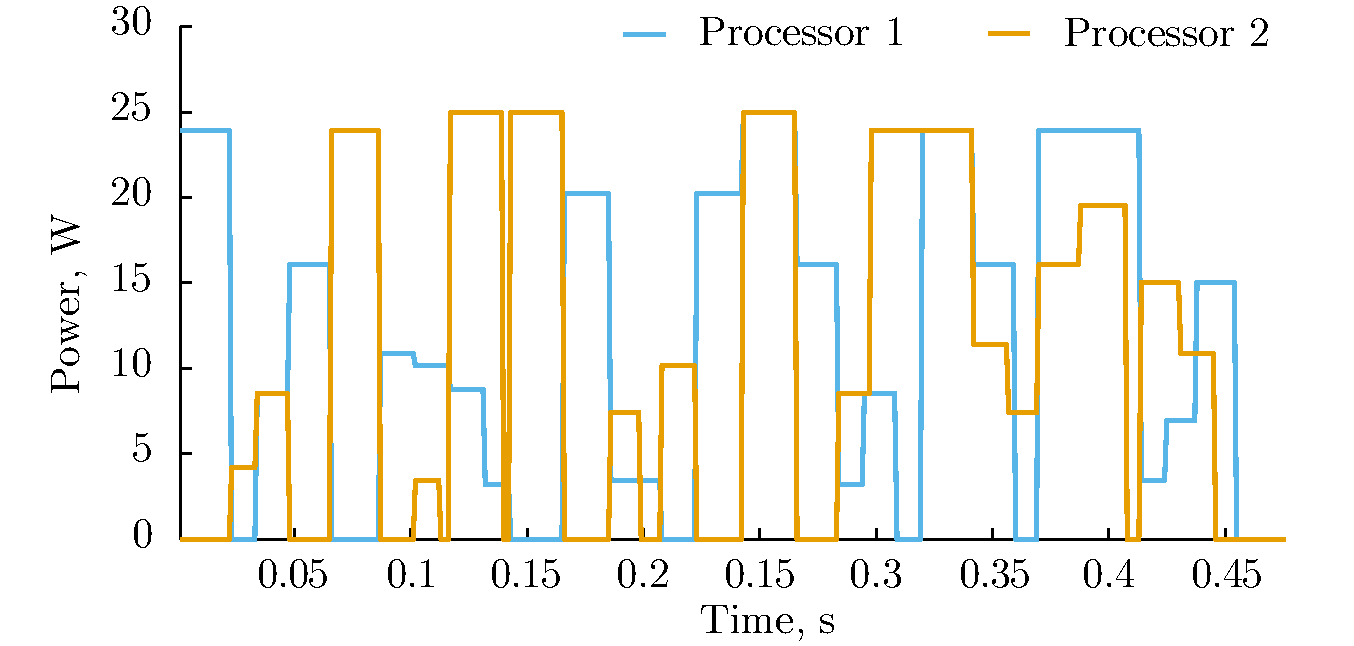
\includegraphics[width=0.90\columnwidth]{include/assets/application-power.pdf}
  \caption{A dynamic power profile.}
  \flabel{power}
  \vspace{-1.5em}
\end{figure}

\begin{figure}
  \centering
  \updatedFigure{
  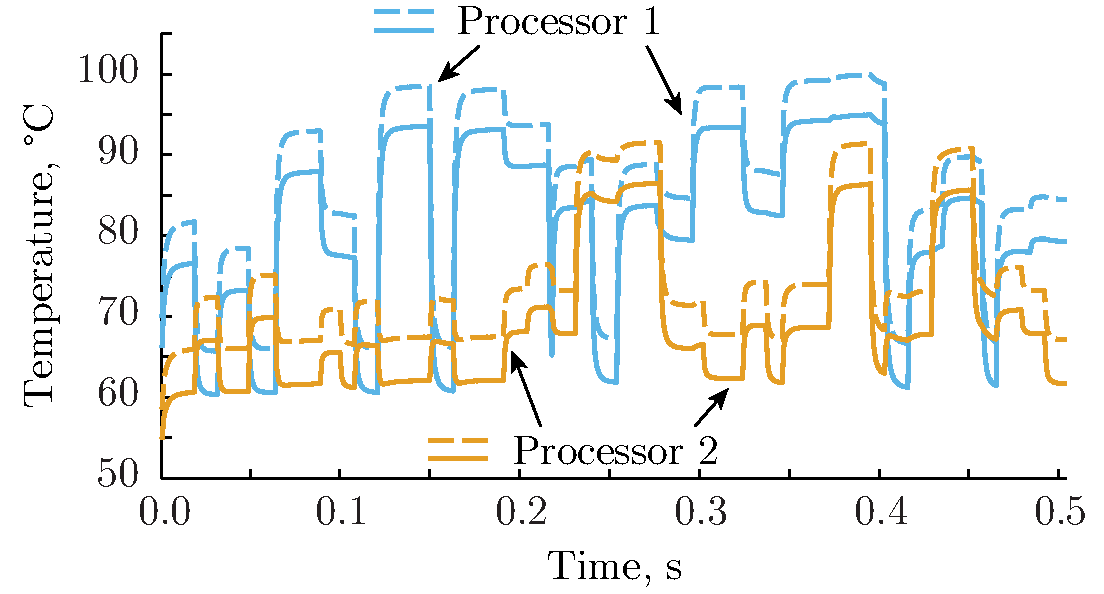
\includegraphics[width=0.90\columnwidth]{include/assets/application-temperature.pdf}
  }
  \vspace{-1.0em}
  \caption{The expected temperature (the solid lines) and one standard deviation above it (the dashed lines).}
  \flabel{application-temperature}
  \vspace{-1.0em}
\end{figure}

\begin{table*}
  \vspace{-0.5em}
  \centering
  \caption{Error measurements for various Monte Carlo samples \textnormal{$\nsamples$} and polynomial orders \textnormal{$\pcorder$}}
  \vspace{-0.5em}
  \begin{tabular}{=c-r-r-r-r-r-r-r-r-r-r-r-r}
    \toprule
    {} & \colExp & \colExp & \colExp & \colExp & \colVar & \colVar & \colVar & \colVar & \colPDF & \colPDF & \colPDF & \colPDF \\
    $\pcorder$ & \colMC{2} & \colMC{3} & \colMC{4} & \colMC{5} & \colMC{2} & \colMC{3} & \colMC{4} & \colMC{5} & \colMC{2} & \colMC{3} & \colMC{4} & \colMC{5} \\
    \cmidrule(r{5pt}){1-1}
    \cmidrule(r{5pt}){2-5}
    \cmidrule(r{5pt}){6-9}
    \cmidrule{10-13}
    \morecmidrules
    \cmidrule(r{5pt}){1-1}
    \cmidrule(r{5pt}){2-5}
    \cmidrule(r{5pt}){6-9}
    \cmidrule{10-13}
    1 & 10.88 & 11.48 & 8.85 & 8.83 & 1.70 & 0.92 & 0.51 & 0.48 & 88.19 & 55.73 & 55.57 & 53.08 \\
    2 & 10.15 & 10.11 & 6.26 & 6.04 & 1.36 & 0.58 & 0.20 & 0.18 & 67.66 & 23.30 & 23.05 & 19.64 \\
    3 &  5.49 &  5.04 & 2.95 & 2.73 & 1.26 & 0.49 & 0.15 & 0.14 & 61.16 & 13.06 & 12.78 &  9.08 \\
    \rowstyle{\bfseries}
    4 &  3.84 &  2.02 & 1.50 & 1.51 & 1.23 & 0.45 & 0.14 & 0.14 & 58.49 &  8.85 &  8.57 &  4.78 \\
    5 &  3.83 &  2.27 & 1.03 & 0.84 & 1.21 & 0.44 & 0.14 & 0.14 & 57.31 &  7.00 &  6.71 &  2.92 \\
    6 &  3.08 &  1.94 & 0.93 & 0.66 & 1.21 & 0.44 & 0.14 & 0.14 & 56.75 &  6.12 &  5.83 &  2.08 \\
    7 &  2.78 &  1.39 & 0.72 & 0.62 & 1.20 & 0.43 & 0.14 & 0.14 & 56.41 &  5.60 &  5.31 &  1.62 \\
    \bottomrule
  \end{tabular}
  \tlabel{accuracy-polynomial-order}
  \vspace{-0.5em}
\end{table*}

We turn to \stage{5}\ in \fref{algorithm}.
It can be seen in \eref{pc-example} that the surrogate model has a negligibly small computational cost at this stage: for any outcome of the uncertain parameters $\vZ(\o) \equiv \vZ$, we can easily compute the corresponding temperature by plugging in $\vZ$ into \eref{pc-example}; the same applies for power.
Consequently, the constructed representation can be trivially analyzed to retrieve various statistics of the system in \eref{fourier-system}.
Let us illustrate a few of them using the same example in \eref{pc-example}.
Assume that the dynamic power profile, $\profilePdyn$, corresponding to the considered workload is the one shown in \fref{application-power}.
Having constructed the surrogate with respect to this profile, we can then rigorously estimate, say, the \pdf\ of temperature at some $k$th moment of time by sampling the surrogate and obtain curves similar to those in \fref{motivation-pdf}.
Furthermore, the expectation and variance of temperature are calculated as simply as (see \eref{pc-moments})
\[
  \oExp{\vTO_k(\o)} = \pcc{\vTO}_{k1} \hspace{1em} \text{and} \hspace{1em} \oVar{\vTO_k(\o)} = \sum_{i = 2}^{6} \pcn_i \: \pcc{\vTO}_{ki}^2
\]
where $\pcn_i$ are normalization constants, and the squaring should be understood element-wise.
For the whole time span of the power profile $\profilePdyn$ depicted in \fref{application-power}, these quantities are plotted in \fref{application-temperature}.
The displayed curves closely match those obtained via MC simulations with $10^4$ samples; however, our method takes less than a second while MC sampling takes more than a day as we shall see next.
